\chapter{Systematics}
\label{sec:Systematics}

In this section studies on systematic uncertainties are discussed.
These cover the signal yields as well as the efficiencies.

\section{Branching ratio uncertainty of subsequent decays}
Regarding equation (\ref{eq:R}) a precise knowledge of the subdecays' \DToKpi and \LcTopKpi branching ratios is essential for the determination of \R.
The values used in this analysis are taken from PDG \ref{PDG} for \BR(\DToKpi) and from a recent \belle measurement \ref{Belle_BR_LcTopKpi} for \BR(\LcTopKpi).
They are
\begin{align*}
    \BR(\DToKpi) &= \BRDToKpival \pm \BRDToKpisysterr, \\ 
    \BR(\LcTopKpi) &= \BRLcTopKpival \pm \BRLcTopKpisysterr.
\end{align*}
Their errors goes in as systematic in the calculation of \R.
They correspond to a relative systematic uncertainty of \SystBRDToKpipercent\% respectively \SystBRLcTopKpipercent\%.

\section{Kinematic \pt(\Lb) reweighting of signal and normalisation channel simulation sample}
To account for the wrong emulation of the \Lb kinematics in the simulation, both, the \LbToDpmunuX and the \LbToLcmunu simulation have been reweighted in the transverse momentum of the \Lb.
Compared to the reweighting of the \LbToDpmunuX decay model this is a minor correction and it is thus sufficient to compare the efficiency ratio \effRatio with and without the kinematic \pt(\Lb) reweighting.
The difference between both cases is used as systematic uncertainty and amounts to $\SysteffRatiokinrew$ corresponding to $\SysteffRatiokinrewpercent\%$.


\section{Reweighting of \LbToDpmunuX simulation decay model}
\subsection{Choice of reweighting dimensions}
As it is not obvious which variables are the best for the reweighting of the \LbToDpmunuX simulation sample to determine the efficiency, they choice of a certain set of weighting variables is absolutely another source of systematics on the final result.
Having a closer look at the comparisons between data and reweighted simulation (see fig. \ref{fig:reweight_D0p_app}) one might argue, that both distribution still aren't in good agreement regarding the particles' momenta.
Thus, another thredimensional weighting in the momenta of the \Dz\proton\mun, \Dz\mun and \Dz candidates is performed and compared with the nominal reweighting.
The difference in the efficiencies \effDp is $\SysteffDpDprew$ or $\SysteffDpDprewpercent\%$.

\subsection{Number of bins per dimension}
To reweight the data the three dimensions are furthermore binned.
Each dimension has been split up in 20 bins.
It is thus interesting to see, how strong the efficiency depends on the choice of the bin number.
For this purpose the reweighting is redone for a variety of different bin numbers.
The results of the efficiency \effDp and the difference to the nominal reweighting can be seen in table \ref{tab:systematic_effD0p_nbins}.
A binning with 5 bins per dimension is too coarse to satisfy the behaviour of the three dimensions.
Using 40 bins per dimension there are too many vanishing weighting bins where there isn't either some data or simulation, hence pulling the other one down and distorting the reweighting.
This can be nicely seen in figure \ref{fig:reweighting_nbins}.
As systematic uncertainty the biggest deviation except for the reweighting with 5 or 40 bins per dimension is assigned, namely $\SysteffDpnbinspercent\%$
 
\begin{table}[tb]
    \centering
    \caption{Comparison of the efficiency \effSelDp for different numbers of bins in each dimension.}
    \label{tab:systematic_effD0p_nbins}
    $\begin{array}{r|r@{\pm}l|c|r}
    \hline
    \text{\# bins}  & \multicolumn{2}{c|}{\effSelDp}  & \text{difference to nominal reweighting} & \text{in \%} \\ \hline \hline
5 & (9.2 & 0.15) \cdot 10^{-3} & \num[round-mode=figures, round-precision=3]{0.000893867513509} & 10.77\%\\ 10 & (8.77 & 0.15) \cdot 10^{-3} & \num[round-mode=figures, round-precision=3]{0.000471373232304} & 5.68\%\\ 15 & (8.4 & 0.17) \cdot 10^{-3} & \num[round-mode=figures, round-precision=3]{0.000101756679921} & 1.23\%\\ 20 & (8.3 & 0.17) \cdot 10^{-3} & \num[round-mode=figures, round-precision=3]{0.0} & 0.00\%\\ 25 & (7.99 & 0.18) \cdot 10^{-3} & \num[round-mode=figures, round-precision=3]{-0.000313870153072} & -3.78\%\\ 30 & (7.88 & 0.19) \cdot 10^{-3} & \num[round-mode=figures, round-precision=3]{-0.000418015648779} & -5.03\%\\ 40 & (8.06 & 0.22) \cdot 10^{-3} & \num[round-mode=figures, round-precision=3]{-0.000243686560501} & -2.94\%\\ 
    \hline
    \end{array}$
\end{table}

\begin{figure}[hptb]
	\centering
	\includegraphics[width=0.32\textwidth]{LbToD0p/comparisons/3D/mD0p_mD0mu_mD0pmu/5Bins/20.0MaxWeight/Bh_DELTA_MASS}
	\includegraphics[width=0.32\textwidth]{LbToD0p/comparisons/3D/mD0p_mD0mu_mD0pmu/5Bins/20.0MaxWeight/B_M}
	\includegraphics[width=0.32\textwidth]{LbToD0p/comparisons/3D/mD0p_mD0mu_mD0pmu/5Bins/20.0MaxWeight/Bh_M} \\
	\includegraphics[width=0.32\textwidth]{LbToD0p/comparisons/3D/mD0p_mD0mu_mD0pmu/10Bins/20.0MaxWeight/Bh_DELTA_MASS}
	\includegraphics[width=0.32\textwidth]{LbToD0p/comparisons/3D/mD0p_mD0mu_mD0pmu/10Bins/20.0MaxWeight/B_M}
	\includegraphics[width=0.32\textwidth]{LbToD0p/comparisons/3D/mD0p_mD0mu_mD0pmu/10Bins/20.0MaxWeight/Bh_M} \\
	\includegraphics[width=0.32\textwidth]{LbToD0p/comparisons/3D/mD0p_mD0mu_mD0pmu/20Bins/20.0MaxWeight/Bh_DELTA_MASS}
	\includegraphics[width=0.32\textwidth]{LbToD0p/comparisons/3D/mD0p_mD0mu_mD0pmu/20Bins/20.0MaxWeight/B_M}
	\includegraphics[width=0.32\textwidth]{LbToD0p/comparisons/3D/mD0p_mD0mu_mD0pmu/20Bins/20.0MaxWeight/Bh_M} \\
	\includegraphics[width=0.32\textwidth]{LbToD0p/comparisons/3D/mD0p_mD0mu_mD0pmu/30Bins/20.0MaxWeight/Bh_DELTA_MASS}
	\includegraphics[width=0.32\textwidth]{LbToD0p/comparisons/3D/mD0p_mD0mu_mD0pmu/30Bins/20.0MaxWeight/B_M}
	\includegraphics[width=0.32\textwidth]{LbToD0p/comparisons/3D/mD0p_mD0mu_mD0pmu/30Bins/20.0MaxWeight/Bh_M} \\
	\includegraphics[width=0.32\textwidth]{LbToD0p/comparisons/3D/mD0p_mD0mu_mD0pmu/40Bins/20.0MaxWeight/Bh_DELTA_MASS}
	\includegraphics[width=0.32\textwidth]{LbToD0p/comparisons/3D/mD0p_mD0mu_mD0pmu/40Bins/20.0MaxWeight/B_M}
	\includegraphics[width=0.32\textwidth]{LbToD0p/comparisons/3D/mD0p_mD0mu_mD0pmu/40Bins/20.0MaxWeight/Bh_M} 
	\caption{Comparison of data (black points) and simulation for the \LbToDpmunuX channel before (red line) and after (red shaded area) threedimensional reweighting as described in the text (see sec. \ref{sec:Reweight_D0p}) for different number of bins per dimension namely 5, 10, 20, 30, 40 bins per dimension from top row to bottom row.}
	\label{fig:reweighting_nbins}
\end{figure}

\subsection{Maximum allowed weight}
The shrinken the impact of single outlier events, a maximum allowed weight of 20 has been defined in the reweighting process.
All events with a higher weight are weighted with this maximum weight.
Analogously to the study of the reweighting in different bins per dimension, a check of the efficiencies obtained by different maximum weights is done.
The results can be seen in \ref{tab:systematic_effD0p_maxweight}.
Again, a maximum weight of 5 is a too tight restriction since there are too many events with weights $> 5$.
Apart from that the biggest discrepancy to the nominal case is taken as systematic uncertainty.
The impact on \R due to the allowed maximum weight amounts to $\SysteffDpmaxweightpercent\%$

 
\begin{table}[hptb]
    \centering
    \caption{Comparison of the efficiency \effSelDp for different allowed maximum weights.}
    \label{tab:systematic_effD0p_maxweight}
    $\begin{array}{r|r@{\pm}l|c|r}
    \hline
    \text{maximum weight}  & \multicolumn{2}{c|}{\effSelDp}  & \text{difference to nominal reweighting} & \text{in \%} \\ \hline \hline
5 & (8.79 & 0.15) \cdot 10^{-3} & \num[round-mode=figures, round-precision=3]{0.000483640507719} & 5.8\%\\ 10 & (8.4 & 0.16) \cdot 10^{-3} & \num[round-mode=figures, round-precision=3]{9.60100390259e-05} & 1.2\%\\ 15 & (8.32 & 0.17) \cdot 10^{-3} & \num[round-mode=figures, round-precision=3]{2.00375500349e-05} & 0.2\%\\ 20 & (8.3 & 0.17) \cdot 10^{-3} & \num[round-mode=figures, round-precision=3]{0.0} & 0.0\%\\ 25 & (8.3 & 0.17) \cdot 10^{-3} & \num[round-mode=figures, round-precision=3]{-5.95559256641e-06} & -0.1\%\\ 30 & (8.29 & 0.17) \cdot 10^{-3} & \num[round-mode=figures, round-precision=3]{-1.05520925512e-05} & -0.1\%\\ 40 & (8.28 & 0.17) \cdot 10^{-3} & \num[round-mode=figures, round-precision=3]{-2.06929754863e-05} & -0.2\%\\ 
    \hline
    \end{array}$
\end{table}


\section{Choice of fit strategy}
The determination of the \LbToDpmunuX signal yield is based on a twodimensional fit in the \Dz\proton mass and the \logIP distribution.
However, actually just the \logIP variable is responsible for the distinction between signal and background.
It should be hence sufficient to fit only the \logIP distribution to extract the signal yield.
As a cross check the signal yield \NDp is determined by a onedimensional fit on the \logIP distribution as described and reported in section \ref{sec:ControlLogIP}. 
The difference between this onedimensional fit and the nominal twodimensional fit amounts to $\SystNDpfit$ events which is equivalent to $\SystNDpfitpercent\%$.

\section{Knowledge of backgrounds}
A limited knowledge of the to the signal yields contributing backgrounds raises another systematic uncertainty.
Different sources of backgrounds have been discussed in section \ref{sec:Backgrounds}.
In the end it is concluded that the background fraction in the obtained signal yield \NDp is $(\NDpBKGratioval \pm \NDpBKGratioerr)\%$.
Propagating the uncertainty on that estimate to the calculation of \R, this means a systematic uncertainty on \NDp due to the limited knowledge of the backgrounds of $\SystNDpBKG$ or $\SystNDpBKGpercent\%$.

\section{Systematics overview}
Table \ref{tab:systematics} summarises all considered systematics and gives a total value for each quantity.
Summing them all up in quadrature to total systematic error on \R is
\begin{align*}
    \Systerr{\R}{} &= \Rsysterr \\
    \frac{\Systerr{\R}{}}{\R} &= \Rsysterrpercent\% 
\end{align*}

 
\begin{table}[hptb]
    \centering
    \caption{Summary of all considered systematics.}
    \label{tab:systematics}
    \resizebox{\textwidth}{!}{
    \begin{tabular}{l||c|c|c|c|c|c|c}
    \hline
    Systematic  & \NDp  & \NLc  & \effDp & \effLc   & \effRatio & \BR(\LcTopKpi) & \BR(\DToKpi) \\ \hline \hline
branching ratios & --- & --- & --- & --- & --- & 3.51\% & 1.29\% \\ 
signal fit & 1.79\% & --- & --- & --- & --- & --- & --- \\ 
backgrounds & 2.85\% & --- & --- & --- & --- & --- & --- \\ 
\Lb \pt reweighting & --- & --- & --- & --- & 1.04\% & --- & --- \\ 
\LbToDpmunuX reweighting & --- & --- & 120.91\% & --- & 120.91\% & --- & --- \\ 
bins per reweighting dimension & --- & --- & 5.68\% & --- & 5.68\% & --- & --- \\ 
maximum weight in reweighting & --- & --- & 1.16\% & --- & 1.16\% & --- & --- \\ 
\hline total & 3.37\% & 0.00\% & 121.05\% & 0.00\% & 121.05\% & 3.51\% & 1.29\% \\ \hline 

    \hline
    \end{tabular}}
\end{table}

